\documentclass{article}
\usepackage[utf8]{inputenc}
\usepackage{graphicx}

\title{Final report}
\author{C group 03(Andy Chen, HouWang Wong, Jeshuran Jebanesan, Jiaju Yang)}

\begin{document}

\maketitle

\section{Abstract}
The aim of this project was to develop a  assembler that decode basic ARM11 assembly language into machine code and an extension  in c programming language. A 2 pass algorithm was implemented for the assembler and as for the extension, it is a 3 player chess game which includes the user interface, chess movement rules and network connectivity to allow multiplayer on local host.
\section{Assembler Structure}
For this program, we use the testing driven approach where we define the tests for the functions first, then define the function. The reason for doing is for the previous project(the emulator), only a few function tests were performed which result in spending long time debugging the program and locating the errors.\newline\newline
As shown in figure 1, the structure was divide into 4 main parts: 
\subsection{Reading and Tokenizing}
    The assemble file was read line by line until the end of the file. The number of words in each line was kept track of. If there was only one word in a line, that line would be a label. If so, the label would be added to the symbol table. If the line was a normal instruction, then the opcode and operands would be stored inside a data structure that would be added onto the end of a linked list.
\subsection{Second pass}
    Going through the linked list of assembly lines with a for loop. Each line was mapped to the corresponding translate function pointer and a default binary. The function is then executed to produce the required binary. This made the functions more independent and making it easier to carry out function testings.
    
\subsection{Translate functions}
    Assembly lines are categorized into 4 main types: data process, data transfer, multiply and branch. A function was defined for each category and translating the assembly line into the corresponding binary code. There were similarity in how different categories of lines are decoded so helper functions are created to reduce code duplication.

\subsection{Output}
    where the binary lines will be converted to little endian format and printed out.
\begin{figure}
\centering
\begin{minipage}{.5\textwidth}
\centering
\includegraphics[width = \linewidth]{ Assembler_structure }
\caption{Assembly structure}
\label{fig:assembly}
\end{minipage}\hfill
\begin{minipage}{.5\textwidth}
\centering
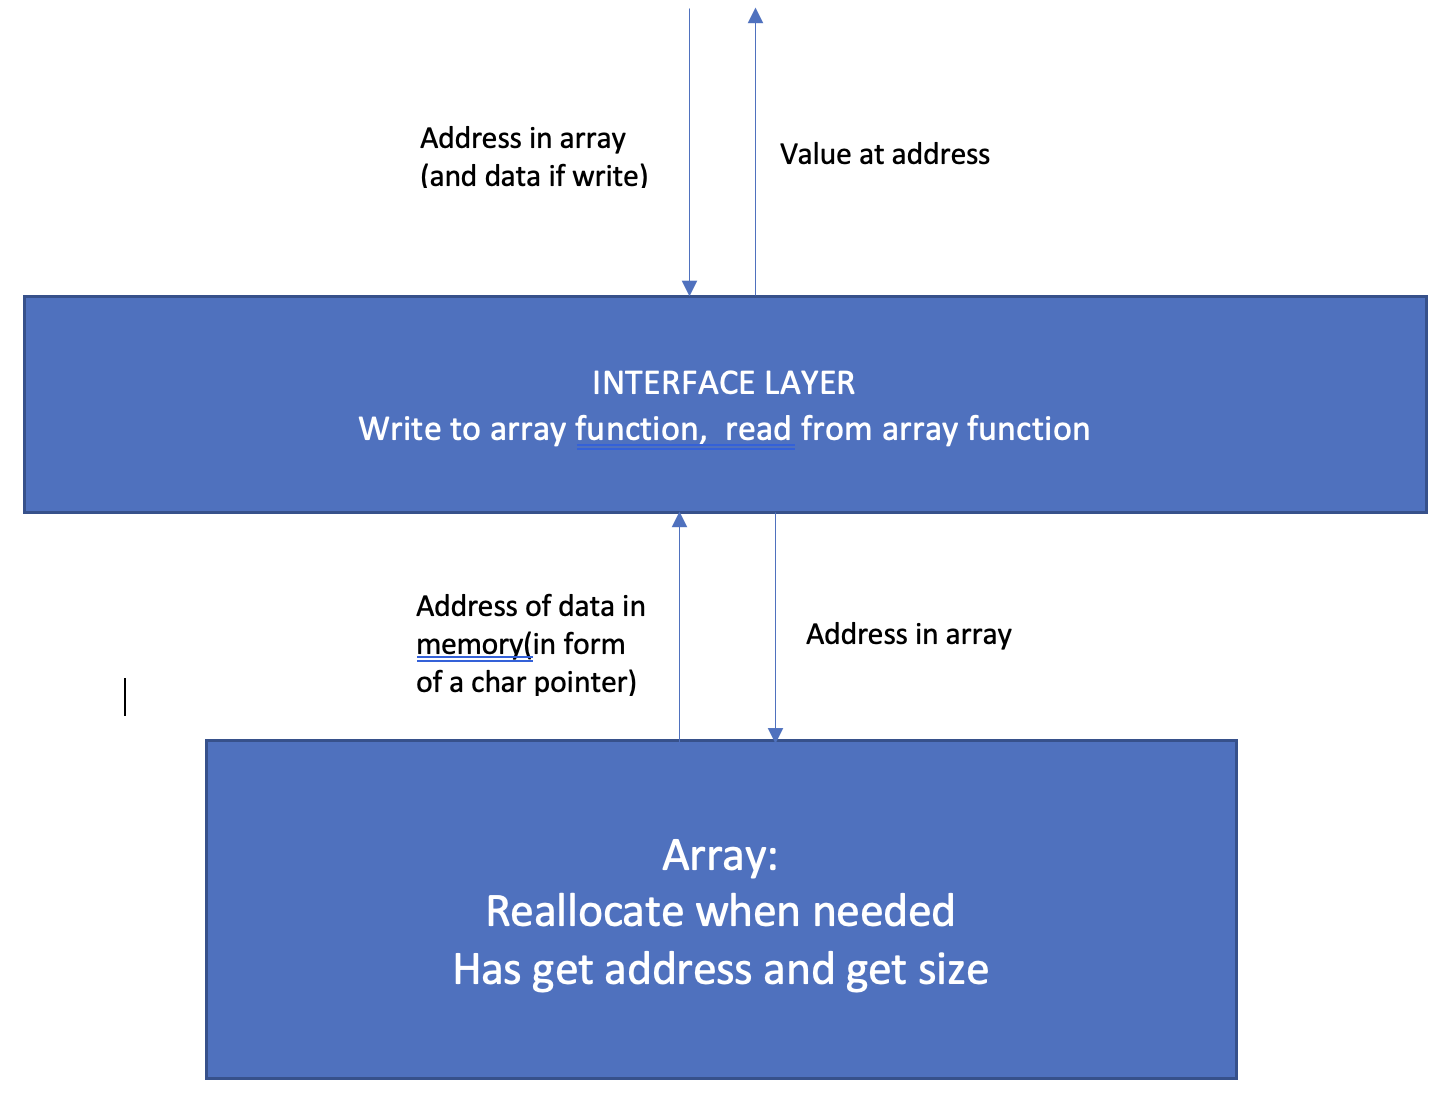
\includegraphics[width = \linewidth]{ mem_array }
\caption{mem array structure}
\label{fig:mem_array}
\end{minipage}
\end{figure}


\section{Challenges}
1.Reading and Tokenizing\newline
    A problem was which data structure to use for assembly lines. The original method was to use a dynamic array. This required the assemble lines to be looped through twice which reduced efficiency. We got around this by using the linked list. Even though a linked list complexity is higher than static array, the assemble lines are read sequentially, which makes the execution time similar to a static array.\newline\newline
    For the symbol table, we used the mem array data structure from the emulator because:
    
    1. The size of array is unknown, which can be solved with mem array's internal automatically reallocate memory function.
    
    2. Mem array can be used to store any type of element. The type conversion will be defined at the interface shown in figure 2.


\end{document}
